\documentclass[onecolumn, draftclsnofoot,10pt, compsoc]{IEEEtran}
%\documentclass[journal, onecolumn, draftclsnofoot, 10pt, letterpaper]{IEEEtran}
\usepackage{listings, import}
\usepackage{graphicx}
\usepackage{url}
\usepackage{setspace}
\usepackage{minted}

\usepackage[justification=centering]{caption}
\usepackage[margin=0.75in]{geometry}
\usepackage{cite}
\usepackage{booktabs}
\usepackage[table,xcdraw]{xcolor}
\lstset{language=c}
\import{./}{stylin.sty}
%\usepackage{geometry}
%\geometry{textheight=9.5in, textwidth=7in}
% 1. Fill in these details
\def \CapstoneTeamName{		Checkmates}
\def \CapstoneTeamNumber{		41A}
\def \GroupMemberOne{			Alex Grejuc}
\def \GroupMemberTwo{			Kai Gay}
\def \GroupMemberThree{			Calvin Gagliano}
\def \GroupMemberFour{			Benjamin Friedman}
\def \CapstoneProjectName{		}
\def \CapstoneSponsorCompany{	OSU College of Engineering}
\def \CapstoneSponsorPerson{		Dr. Martin Erwig}

% 2. Uncomment the appropriate line below so that the document type works
\def \DocType{End-Of-Term Report}
% or others...

\lstset{ % General setup for the package
	language=Haskell,
	basicstyle=\small\sffamily,
	numbers=left,
 	numberstyle=\tiny,
	frame=tb,
	tabsize=4,
	columns=fixed,
	showstringspaces=false,
	showtabs=false,
	keepspaces,
	commentstyle=\color{red},
	keywordstyle=\color{blue}
}
			
\newcommand{\NameSigPair}[1]{\par
\makebox[2.75in][r]{#1} \hfil 	\makebox[3.25in]{\makebox[2.25in]{\hrulefill} \hfill		\makebox[.75in]{\hrulefill}}
\par\vspace{-12pt} \textit{\tiny\noindent
\makebox[2.75in]{} \hfil		\makebox[3.25in]{\makebox[2.25in][r]{Signature} \hfill	\makebox[.75in][r]{Date}}}}
% 3. If the document is not to be signed, uncomment the RENEWcommand below
%\renewcommand{\NameSigPair}[1]{#1}

%%%%%%%%%%%%%%%%%%%%%%%%%%%%%%%%%%%%%%%
\begin{document}
\begin{titlepage}
    \begin{center}
    	
\includegraphics[height=3cm]{img/osu.png}
    \end{center}
    \pagenumbering{gobble}
    \begin{singlespace}
        \hfill 
        % 4. If you have a logo, use this includegraphics command to put it on the coversheet.
        %{\centering 
\includegraphics[height=4cm]{img/osu.png}}   
        \par\vspace{.2in}
        \centering
        \scshape{
            \huge CS Capstone \DocType \par
            {\large\today}\par
            \textbf{\Huge\CapstoneProjectName}\par
            {\large Prepared for}\par
            \Huge \CapstoneSponsorCompany\par
            \vspace{5pt}
            {\large Prepared by }\par
            \vspace{5pt}
            {\Large    
                Group\CapstoneTeamNumber\par
                \CapstoneTeamName\par
                \vspace{14pt}
            {\Large
                Alex Grejuc, Kai Gay, Calvin Gagliano, Benjamin Friedman
            }\par
            {\Large Winter 2019}\par
            \vspace{20pt}
            }
        }
        \begin{abstract}
          Domain Specific Languages (DSLs) can be used in a myriad of applications. In particular they are useful for teaching Computer Science concepts to new students. By learning to work with a DSL, students can focus on a smaller domain, which means they can become more comfortable and less overwhelmed by the topics that are introduced through that DSL. Still, most early students have trouble learning their first computer language, regardless of scope, as it introduces a new approach to thinking. To improve on this issue, and to still teach computer science concepts early on, our approach was to design and implement a DSL that can help students learn algorithms by describing board games. By focusing on a specific subset of games with 2D boards, we find that algorithms, logic, and program flow can be derived from most students' preexisting understanding of board games. We have successfully designed this DSL, and are in the midst of completing the finishing touches on it. We also have a web-based user interface that we describe as a means to improve the quality of user's interactions with our language. We present our work so far on implementing this language, as well as our current project state, outstanding work, past and present problems, code selections and results from our research into developing this DSL.
        \end{abstract}    
    \end{singlespace}
\end{titlepage}
\newpage
\pagenumbering{arabic}
\tableofcontents
% 7. uncomment this (if applicable). Consider adding a page break.
%\listoffigures
%\listoftables
\clearpage

\begin{singlespace}

\section{Project Recap}
    We are designing and implementing Spiel, an educational domain specific (programming) language (DSL), for the specification of board games. In addition to the language itself we will be creating an interpreter, a syntax-directed editor, and a graphical interface to visualize the games. Spiel will be used to address the difficulty of early computer science education, specifically for middle school students. 
    
    We chose to implement Spiel as a DSL because the simplified domain streamlines the process of learning to program, and enables students to focus on core concepts (such as looping or abstraction). We chose the domain of board games because it is one that middle school students can have fun thinking about and/or already have a strong intuition for. Within the domain of board games we further limit the types of games we are interested in describing to 2D rectangular board games that play with some aspect of territorial acquisition.
    
    The end goal of our project is to produce this language and to be able to distribute it to teachers so that students can learn with it. This means providing an easy to understand (and multi-platform) interface such that users on OSX, Linux, or Windows will be capable of using our language successfully. In addition, our goals include providing some informative material with our language, such that existing lessons are available for teachers and new lessons can be easily added.
    
\section{Project Status}
    %We combined the ideas of multiple draft versions of board game languages (syntax and semantics) into a single draft language, which we expect to be close to the final version. We have implemented the first version of a parser for this language, which is able to parse concrete syntax specifications of tic-tac-toe and Connect Four into an abstract syntax. We need to verify that this parser is correct through tests with other game specifications, and to then begin working on the evaluation function for the semantic aspect of our language. Once we are at this point, we will begin working on the syntax-directed editor and graphical components of our project.
    At our current project state we have settled on a syntax and semantics, choosing to do something similar to Haskell, with some quality of life changes \cite{bogl}. In particular we have stripped down the syntax to only what is absolutely necessary to achieve our goal of teaching early computer science concepts. This involves leaving out such things as Lists and Strings, which although very common in other languages, are purely extraneous to our goal. 
    
    Currently, we have a parser, typechecker, and evaluator completed for the language. The parser takes BoGL files (usually ending in .bgl), and reads over them to produce an abstract syntax tree that is representative of the program. During this process we can report parser errors that occur from invalid syntax. These kinds of feedback are then displayed to the user in the read evaluate print loop (Repl), or passed along to be displayed on the frontend by our server (which will be detailed below). Upon sucessful parsing, the typechecker goes over our parsed syntax, and then verifies that the abstract syntax produced is type correct. Since our language is strongly typed, we do not allow ambiguous types, and we return type checker errors if an expression receives a value of an invalid type (such as when expecting a Board but receiving a Player). The evaluator then runs on this abstract syntax to perform the intended actions encoded in our language. The results of this evaluation are then returned to the user, where they can again supply further input.
    
    We have a friendly editor and user interface provided by a react frontend. This provides an interface via a website that can be visited by any browser, and provides an editor and a Repl. Code can be pasted into the editor, and it can be saved by typing commands into the Repl. Arbitrary commands can be executed from the Repl as well (such as starting a game), allowing this web-Repl to function very similarly to a normal Repl in the terminal/command prompt.
    
    Currently we are at a point where work on user and developer-level documentation is becoming very important. This will allow future work on our project to be done by other developers, as well as enabling the teachers who will use this language to better understand the material they are presenting. In addition, more examples and guides are necessary. We will be receiving feedback from the client through the GitHub issues page, which will allow us to quickly work on any issues instructors or students have.
    
    We have implemented a language server as part of Spiel. This allows us to quickly startup a backend that has a fixed API to accept JSON data via REST requests. These are standard requests that are performed for accessing resources across the internet, and this allows us to keep the frontend from being tightly coupled with the backend. The frontend only needs to be aware of the exposed REST endpoints, where it can make specific requests for saving data, running commands, playing a game, making a move in a game, or restarting a game. The frontend does not need to know how these requests are performed, it simply asks that they be done with input provided from the user. If the requests are invalid, the backend will handle it, and return a proper response to the frontend in JSON.
    
    With all these components combined, we have a functional system that is at a Beta state. It is capable of being interacted with to write board descriptions, run commands, play games, and get feedback regarding syntax or type errors (see figure \ref{fig:r1}).
    
    \begin{figure}
        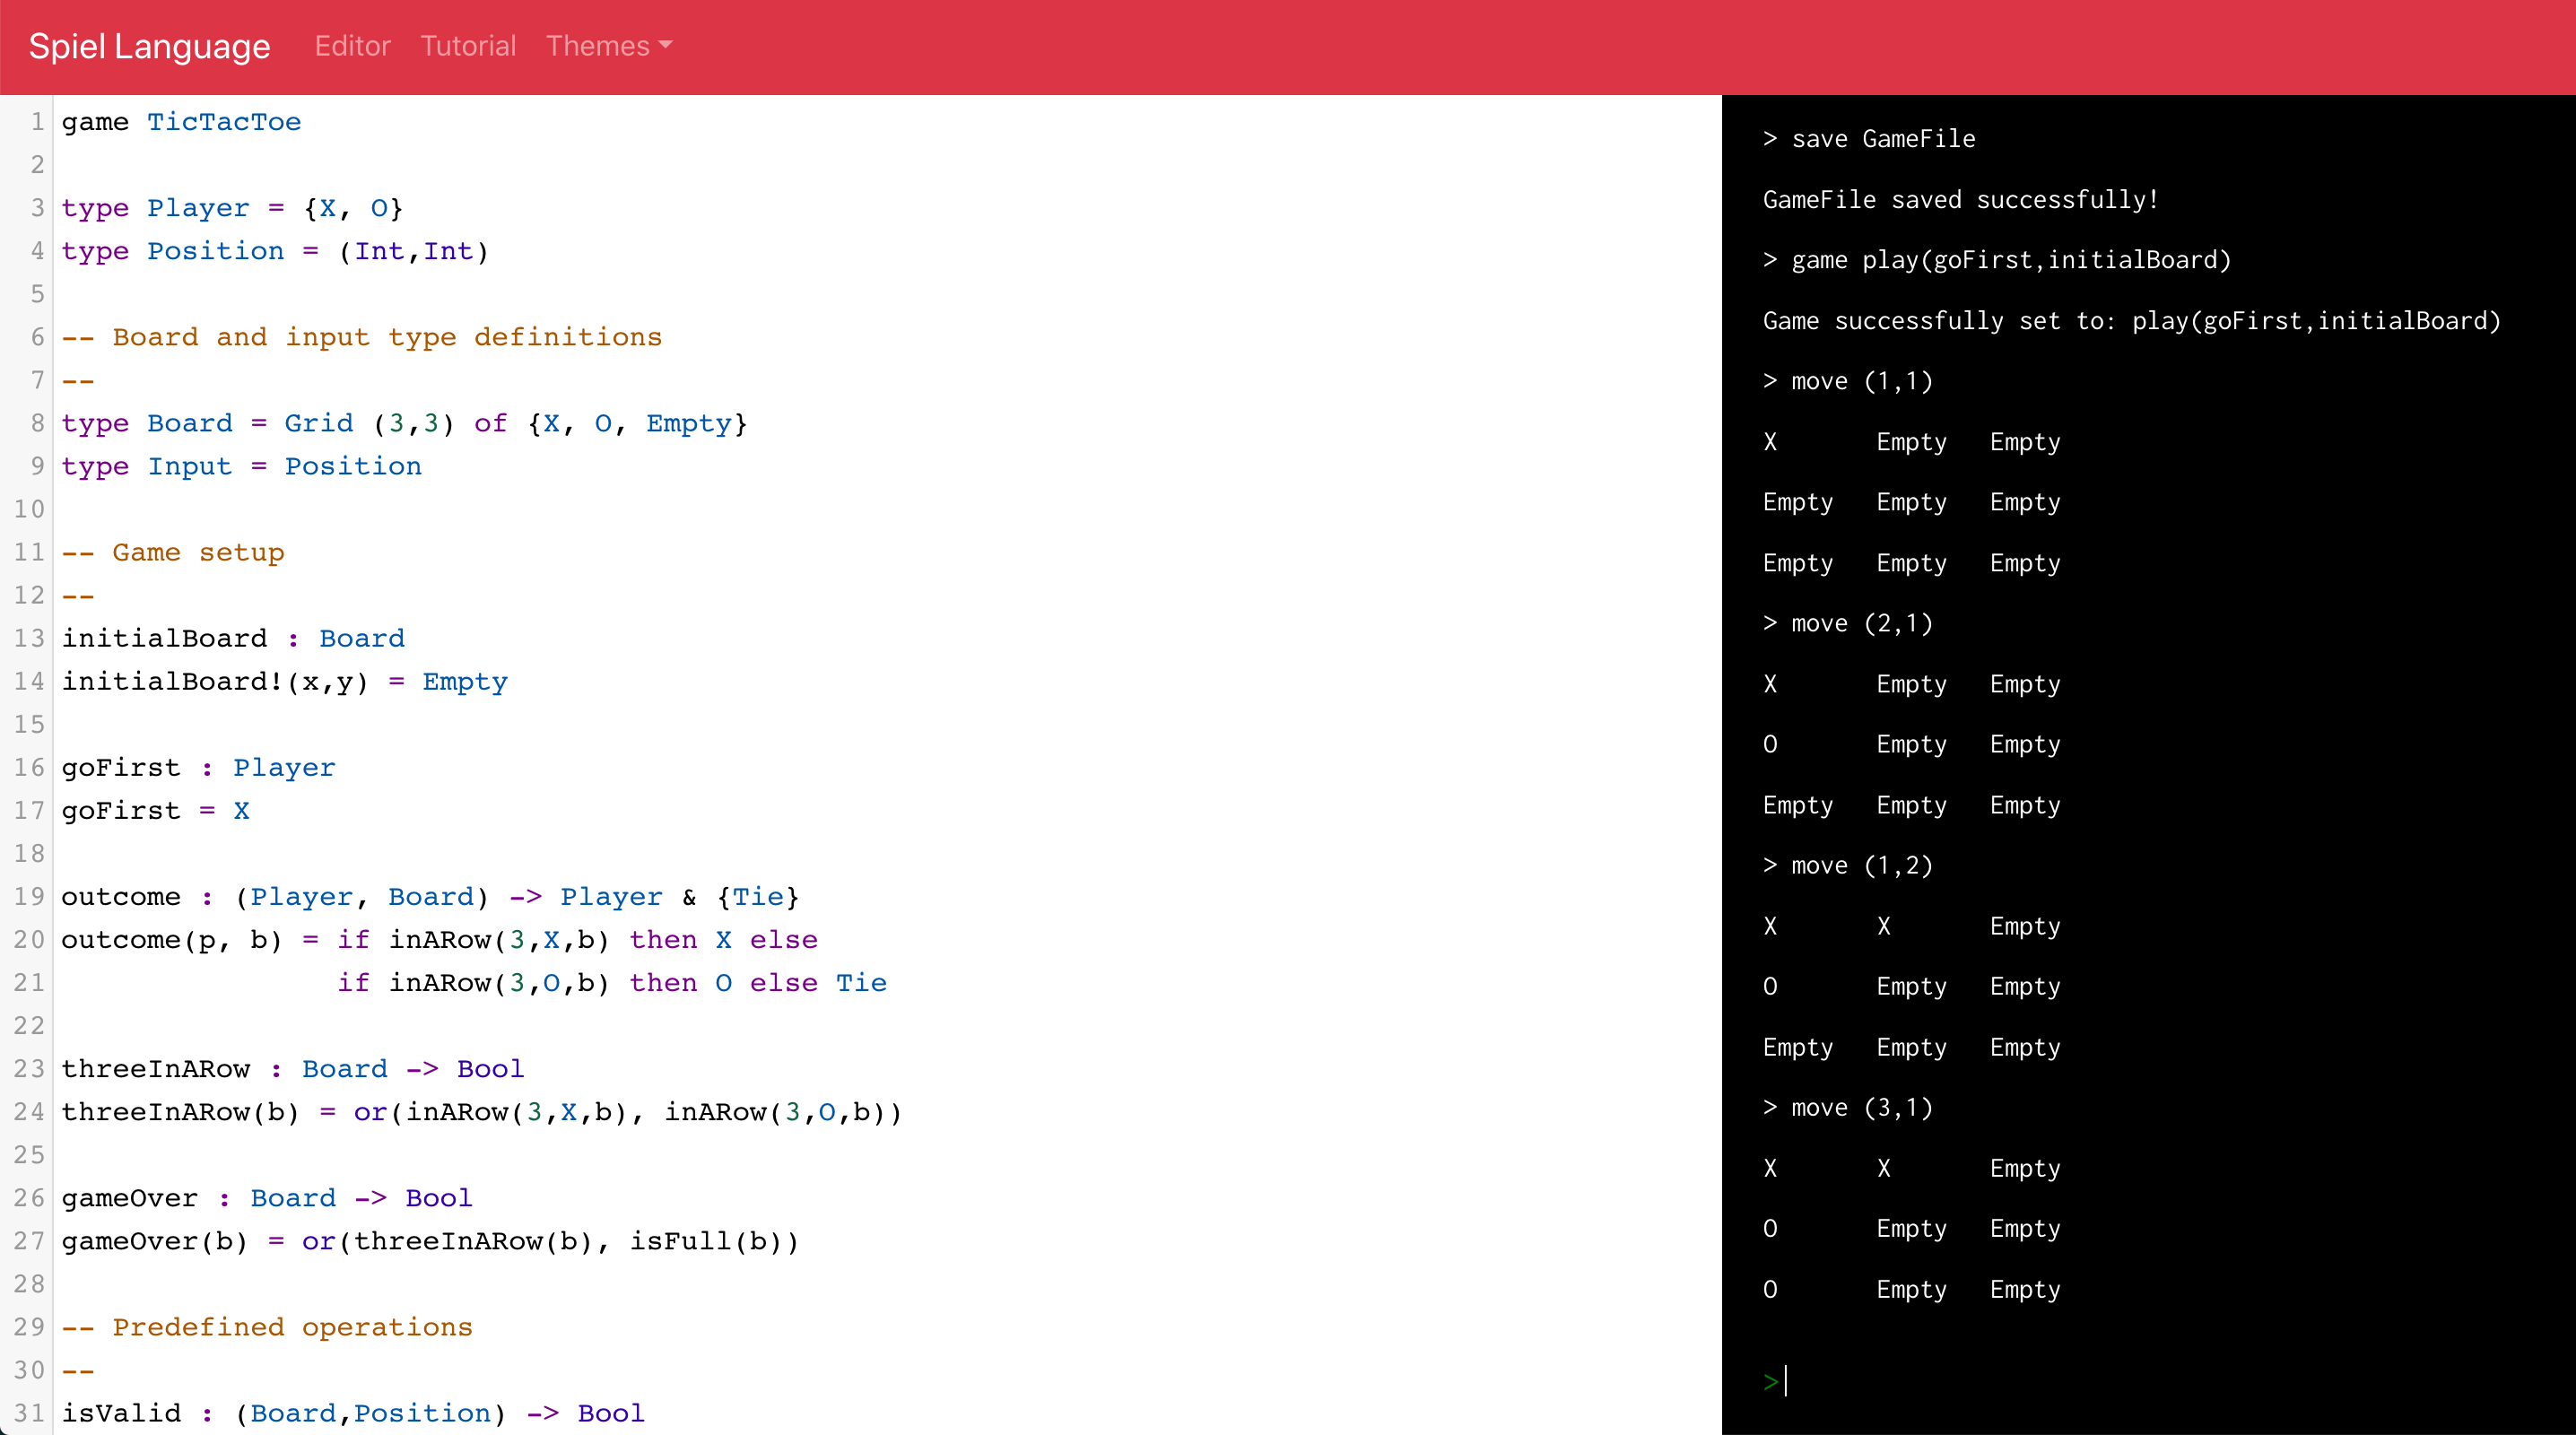
\includegraphics[width=1.0\textwidth,keepaspectratio]{./img/p1}
        \caption{A view of the web-based editor and Repl, loaded up with code to describe a game of TicTacToe. See also on the right the results of running invididual commands in the Repl.}
        \label{fig:r1}
    \end{figure}
    
\section{Outstanding Work}
    Before we are ready to deliver our project, and to consider it done, we still need to have user tests and platform-specific packages ready (as mentioned above). In particular, we need to provide packages that are reliably cross-platform in nature, and do not require more than what is provided in the package. This can be done in Haskell for our language via static compilation, but must be done once for each platform we want to distribute for. In addition, our user facing interface (frontend) can be distributed as an electron application, but this too must be carefully produced to work on specific platforms.
    
    We still have to work on some syntax-directed editing, allowing the typechecker to provide hints in the editor, tab completion, and better error reporting. All of these are being worked on across both the frontend and backend of our project. The outstanding issue with error reporting is that we need to send back the line number, column number, and associated error message in the response from the backend. The frontend then needs to take this information, and informatively update the editor window to highlight the error. This needs to be done for both syntax and type checker errors, and they should update when corrections are made.
    
    Usage level documentation still needs to be produced. We plan to do this in two ways: introducing the concepts of installing, running, and working with the frontend itself, and to have documentation regarding how to write actual board game descriptions. The later of these 2 will be significant as it will be a reference point for producing lesson plans that students can then follow. It is likely that instructors will want to curtail their lessons to the students they are teaching, and so they need to be familiar enough with the language to make the changes they want.
    
    In addition, language level documentation still needs to be produced (via Haddock) for the implementation of our DSL itself. This will serve to inform us and future developers how to work on, maintain, and modify our code base without breaking the core functionality of our program. As an extended part of this, the existing test cases (which do work, and are present) need to be bolstered to provide a means of verification of project integrity after making changes. There have been some issues with this, but we will detail that in the following section.
    
    The frontend of our application needs some additional work, as it currently has only the editor and Repl in place. The frontend will also need tutorials, and user level documentation for those who are learning the language. We expect this to be one of the last things that we implement, as it can only be done properly once the language itself has been solidified, and will not experience further changes.
    
    We also need to have our project tested by other users. This involves preparing a 'one-click' install version of our language, complete with backend and frontend components. We are currently in the midst of putting together this package, and expect to have this ready soon to deliver for testing purposes. In addition our current editor is still a beta draft, so it will require further refinement based on the input we receive from our client.
    
\section{Project Impediments}
    One major problem is our relative inexperience with more advanced Haskell concepts (monads, applicatives, etc) and libraries (Parsec) which are useful for our implementation. We are solving this problem by having everyone implement some features completely on their own (everyone in the group created an abstract syntax and evaluation function which could at least model tic-tac-toe). We continue to share knowledge and tutorials within our group, and each of us are filling in gaps as needed. 
    
    The other major problem we had is back and forth progress on the design of our language, which is to be expected given the inherent lack of clarity that comes with research-oriented projects. In particular, we have wavered on concepts and features in the design of our language (e.g. implicit versus explicit loops, support for different types of pieces, a declarative versus imperative paradigm, etc). These are philosophical issues which cannot be quantified, so we spent a long time debating them. This made it difficult to start implementing features early on. To resolve this, we agreed that our client would decide on the final syntax and features of the language. He has since given us a concrete syntax and semantics which we expect to be close to the final version of our language, and we have implemented the majority of it already. 

    We have also had an issue with lack of clarity as to the environment where our language (backend and frontend) will be used. We understand that it will be used in summer camps to help teach early computer science topics (such as algorithms to students), but we have not been informed the format of the learning experience. We have also not been told as to what kind of computers they will be working with, and so we haven't been able to determine exactly what platforms we should be focusing on. As a result, designing packages for end user applications must be done generally and for the primary 3 platforms we could probably expect (OSX, Linux, Windows). There is also the distinct possibility that the summer camps where this language will be used may be cancelled, given the global pandemic of COVID-19. Although this will likely not impact our deadline requirements, it may prevent our project from ever being applied as intended, at least until Summer of 2021.
    
    Testing has not been performed as thoroughly as we would want. This is in part because breaking changes are frequently introduced into the language, which is the nature of a research based project. However, this has been an issue as it means that consistency in terms of project validity has been unreliable at best. Without consistent testing we have little to no means of verification, beyond what we check by hand. This is something that we will be fixing by expanding the test suite, but we can only do this once the language has 'cooled down', and breaking changes are no longer introduced by our client. At that point, we anticipate being able to bring our testing up to speed.
    
    Finally, the server can be crashed by invalid response data from the backend. This can be caused by malformed responses inputted by the frontend to the backend, and returns something that is not legitimate JSON. Upon trying to parse this response react will display an error page. Two things need to be done to fix this. The first being that the backend should check for and handle potentially invalid commands, and should return a valid SpielError in JSON format for the frontend to handle. Secondly, the frontend should implement fallback catching on all promise chains that are used to handle AJAX requests to the backend. This means the frontend should be capable of correctly handling invalid feedback from the server after making a request, and should instead tell the user discretely that there was an error in their last command.
    
\section{Code Selections}
The core of the abstract syntax tree is the expression. Haskell allows us to represent expressions in a very elegant way, due to the feature of abstract data types:
\begin{minted}{haskell}
-- Expr Datatype
data Expr = I Integer
          | S String
          | B Bool
          | N Name
          | Tuple [Expr]
          | App Name [Expr]
          | Binop Op Expr Expr
          | Let Name Expr Expr
          | If Expr Expr Expr
          | While Expr Expr
\end{minted}
Another useful feature of haskell is the ease in which we can write concise parsers with the Parsec library. Here is a piece of code using the applicative parser style:
\begin{minted}{haskell}
-- parser fragment
equation :: Parser Equation
equation =
  (try $ (Veq <$> identifier <*> (reservedOp "=" *> expr)))
  <|>
  (try $ (Feq <$> identifier <*> 
  (Pars <$> parens (commaSep1 (identifier))) <*> (reservedOp "=" *> expr)))
  
\end{minted}
Here is an expression in the Spiel language:
\begin{lstlisting}
if inARow(3,A,b) then A else
if inARow(3,B,b) then B else
if isFull(b)     then Tie else Continue
\end{lstlisting}
And here is the parsed statement:
\begin{minted}{haskell}
(If
    (App "inARow" [I 3,N "A",N "b"]) 
    (N "A")
    (If
        (App "inARow" [I 3,N "B",N "b"]) 
        (N "B")
        (If 
            (App "isFull" [N "b"]) 
            (N "Tie") 
            (N "Continue"))))
\end{minted}
Given that our project is a language itself, we thought it prudent to incorporate an example of a fully functioning game as well. In particular we choose to show TicTacToe, a simple game that has been around since at least the time of the Roman Empire \cite{tictactoe_origin}.
\lstinputlisting{TicTacToe.hs}

\section{Research Results}

Our project was predominantly focused around research, the goal of which was to discern an appropriate abstract and then concrete syntax by which to design our entire DSL around. Our initial term in Fall found us spending the vast majority of our time debating over this. Ultimately, a concrete syntax (as provided by our client) was decided on and has since been the focus of our development work. Looking back at our research before, we have concluded the following at our current state:
\begin{itemize}
    \item A DSL will be most effective in a limited domain, ideally a familiar domain to the target user group.
    \item Out of the domain of board games, we find that certain board games (such as battleship and life) are too beyond the scope of our goals, and it would behoove us to focus on simpler games instead.
    \item Lists, Strings, and other high-level ubiquitous concepts do not help us to teach algorithms, and introduce more complexity than is desired.
    \item Regardless of the effectiveness of our implementation, usage of this language will only be as effective as the means of introducing it to our target user group (a bad introduction may defeat the purpose of acclimating students).
    \item Requiring definitions to be defined in order may be more conducive to a student learning our language in a linear fashion, rather than using an order in-dependent set of definitions.
\end{itemize}

Many of these results are tentative based on the limited observations we made (consisting of discussions with our group, the other group, and our client), and may change once we deploy our language into actual usage. We anticipate this, but also expect that most of our conclusions are made with reasonable justification to consider them a sound basis to build our DSL on.

\begin{thebibliography}{20}
\bibitem{tictactoe_origin}
Garcia, Dan. "Tic-Tac-Toe". \textit{UC Berkeley}. March 2020. http://gamescrafters.berkeley.edu/games.php?game=tictactoe. Accessed: March 17th, 2020.

\bibitem{bogl}
Erwig, Martin. "BoGL Syntax". \textit{Github}. March 13th, 2020. https://github.com/The-Code-In-Sheep-s-Clothing/Example-DSTL/blob/master/BGL-Syntax.pdf. Accessed: March 17th, 2020.

\end{thebibliography}

\end{singlespace}

\end{document}